\chapter{openPOWERLINK}
\label{cha:oplk}
openPOWERLINK is an Open Source implementation of the POWERLINK protocol.
The implementation contains the openPOWERLINK stack, different demo applications for various platforms and is designed for an simple introduction into POWERLINK.
The available project should allow manufacturers an easily integration of POWERLINK into their projects.
The Open Source implementation should targets an improved integration an development of new features.

%TODO general description of openPOWERLINK

\section{POWERLINK}
\label{sec:powerlink}
POWERLINK is an industrial real-time communication protocol based on the IEEE 802.3 standard (Ethernet \cite{ethernet_ieee_2016}).
POWERLINK was developed by the members of the Ethernet POWERLINK Standardization Group (\emph{EPSG}).
The \emph{EPSG} consists of different companies located in the field of real time communications, automation and field bus communication. \cite{epsg_hp}

%TODO general description of POWERLINK

\subsection{Network structure}
\label{sec:oplk_powerlink_network}
A POWERLINK network consists of the following two different node types.

\begin{description}
    \item[MN] The managing node exist once within a normal POWERLINK network and controls the communication flow.
    The MN manages all registered network participants, provides a clock and defines the transmission cycle.
    \item[CN] All other nodes within a normal POWERLINK network are controlled nodes and react according to the controls of the \emph{MN}.
\end{description}

Within a POWERLINK network unique POWERLINK addresses (Node IDs) are assigned to each node.
The address range from 1 to 239 is available for all \emph{CNs} and can be assigned freely.
The address 240 is fixed for the \emph{MN}, each node assigned the Node ID 240 automatically performs the \emph{MN} functionalities.
\cite{epsg_epsg_2013}

A simple POWERLINK network consisting of a \emph{MN} connected to one \emph{CN} directly and additional two \emph{CNs} via a Ethernet HUB is shown in figure \ref{fig:powerlink_network}.

\begin{figure}
    \centering
    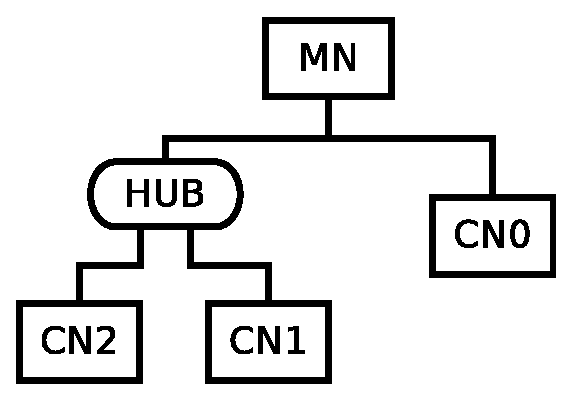
\includegraphics[width=0.5\linewidth]{powerlink_network}
    \caption{POWERLINK network consisting of a \emph{MN} connected to one \emph{CN} and a Ethernet HUB which is connected to two more \emph{CNs}.}
    \label{fig:powerlink_network}
\end{figure}


%TODO describe topologies

\subsection{Frame}
\label{sec:oplk_powerlink_frame}
The POWERLINK frame is embedded in an Ethernet 2 Frames payload and is defined via the Ether type 0x88AB.
Therefore the POWERLINK frame is preceded by the Ethernet 2 Header containing destination \emph{MAC} Address, source \emph{MAC} Address and Ether type.
The payload of an Ethernet 2 Frame can reach up to a length of 1500 bytes succeeding with 4 bytes checksum. \cite[section 3.2]{ethernet_ieee_2016} \cite[section 4.6.1]{epsg_epsg_2013}

In figure \ref{fig:powerlink_frame} the structure of a POWERLINK frame is shown.
The POWERLINK header shown to the left contains the destination and source Node Id preceded by the message type.
The payloads length and content is depending on the transmitted message and thereby defined by the message type. \cite[section 4.6.1.1]{epsg_epsg_2013}

\begin{figure}
    \centering
    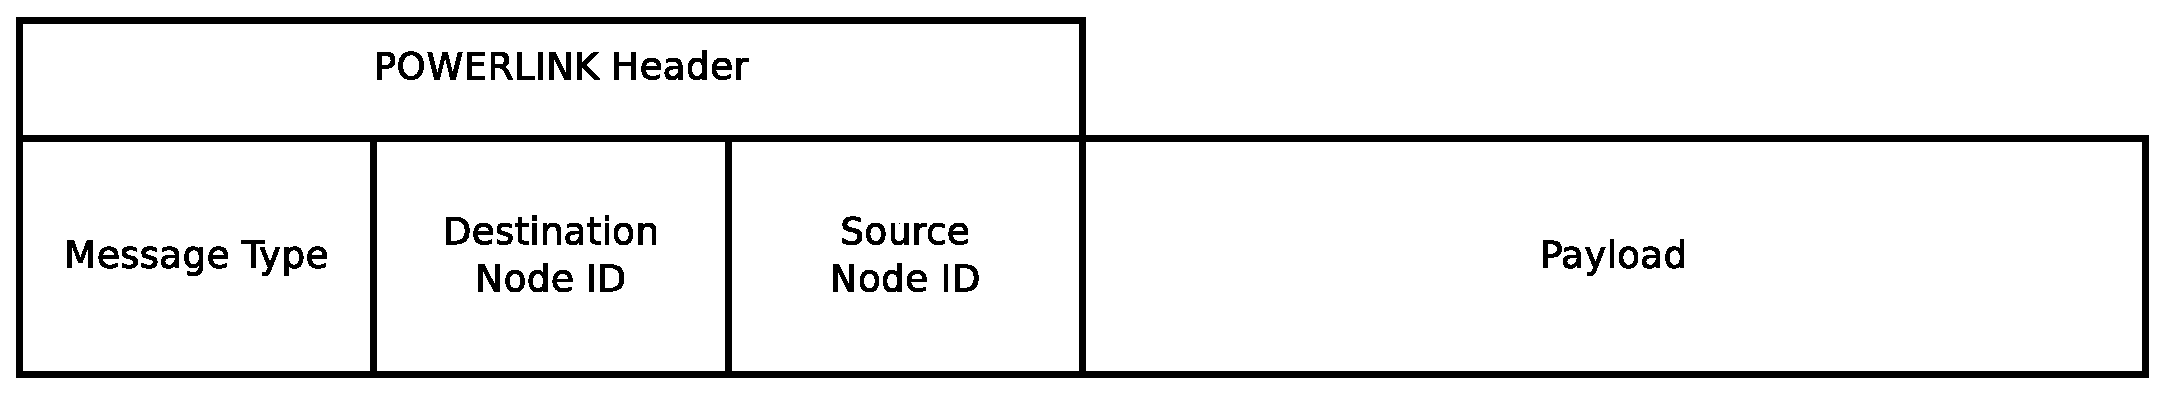
\includegraphics[width=0.9\linewidth]{powerlink_frame}
    \caption{POWERLINK frame showing POWERLINK header and payload.}
    \label{fig:powerlink_frame}
\end{figure}

Detailed information about the different structures of transmitted payloads depending on the message type can be found here \cite[section 4.6.1.1.1]{epsg_epsg_2013}

\subsection{Commands}
\label{sec:oplk_powerlink_commands}

As mentioned above different transmitted POWERLINK messages are defined via the message type.
The following commands are distinguished by the according message type.

\begin{description}
    \item[Soc] Start of cycle is sent by the \emph{MN} as multicast and defines the start of the POWERLINK cycle and the isochronous phase.
    \item[PReq] Poll request is sent by the \emph{MN} to a specific \emph{CN} transmitting data and requesting the transmission data from the \emph{CN}.
    \item[PRes] Poll response is sent by the \emph{CN} as multicast as response to a \emph{PReq} and contains data from the \emph{CN}.
    \item[SoA] Start of Asynchronous is sent by the \emph{MN} as multicast and defines the end of the isochronous phase and the begin of the asynchronous phase.
    \item[ASnd] Asynchronous send is sent either by the \emph{MN} or a \emph{CN} as multicast and contains asynchronous data.
\end{description}

The sequence of sent command within a POWERLINK cycle is shown in the next section.

\subsection{Communication cycle}
\label{sec:oplk_powerlink_commcycle}

The POWERLINK communication cycle is separated in two different phases.

The isochronous phase is the first part of a POWERLINK cycle and is started by the \emph{MN} sending a \emph{SoC} message.
Within this phase the \emph{MN} is polling each \emph{CN} with registered isochronous data.
This polling is accomplished via sending \emph{PReq} message to each \emph{CN}.
This message includes information for the \emph{CN} and also isochronous data which should be sent from the \emph{MN} to the specific \emph{CN}.
After the reception of the \emph{PReq} message the \emph{CN} is sending a \emph{PRes} message as multicast.
This message includes all isochronous data which is requested by the \emph{MN} or any other \emph{CN}.
By multicasting this message each node which should receive a specific data set is immediately receiving the new values. \cite[section 4.2.4.1.1]{epsg_epsg_2013}

When the last isochronous \emph{CN} sent its \emph{PRes} message the isochronous phase is over.
The end of this phase and the start of the asynchronous phase is marked by the sent \emph{SoA} message by the \emph{MN}.
This message contains information about the node which is assigned to the current asynchronous slot.
In each cycle the \emph{MN} assigns the asynchronous slot to either itself or to a \emph{CN}.
Additionally the requested service is transmitted.
Demands a \emph{CN} the assignment to a asynchronous slot this must be communicated to the \emph{MN} either by the \emph{PRes}, \emph{IdentResponse} or \emph{StatusResponse} message.
The communicated number of pending asynchronous messages can additionally provide a priority for better scheduling. \cite[section 4.2.4.1.2]{epsg_epsg_2013}


In figure \ref{fig:powerlink_cycle} a simple POWERLINK communication cycle is shown.
Above the horizontal time axis all command sent by the \emph{MN} are shown.
Commands sent by different \emph{CNs} are displayed below the axis.
This communication cycle shows the isochronous phase marked by the dotted box to the left.
This phase includes the starting command \emph{SoC} and the sequential polling of each \emph{CN}.
This example matches the shown network in figure \ref{fig:powerlink_network} and contains three \emph{CNs}.
The different \emph{CNs} are immediately responding to the polling request.

At the right side in figure \ref{fig:powerlink_cycle} the asynchronous phase is marked by the dashed box.
The asynchronous phase contains the \emph{SoA} command  and following asynchronous data transmission.

\begin{figure}
    \centering
    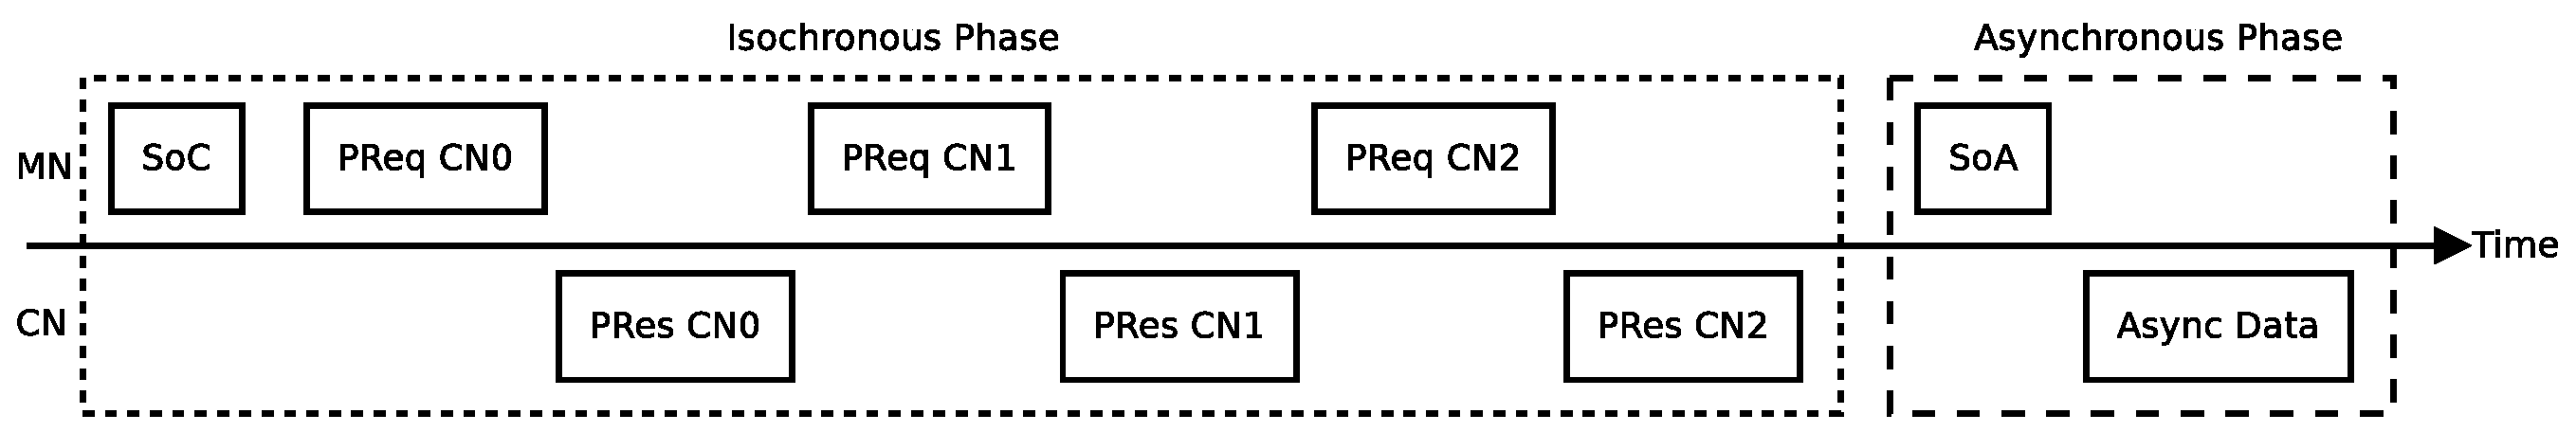
\includegraphics[width=0.95\linewidth]{powerlink_cycle}
    \caption{POWERLINK communication cylce containing Isochronous Phase with polling of three \emph{CNs} and Asynchronous Phase.}
    \label{fig:powerlink_cycle}
\end{figure}

\subsection{Data transmission}
\label{sec:oplk_powerlink_data}


\section{Structure}
\label{sec:oplk_structure}
The openPOWERLINK stack distribution package is structured in different main directories containing demo applications, documentation, driver implementation, the stack sources and multiple more.

For this paper the most important parts are the stack sources and demo applications..
Furthermore an additional simulation directory will be added whose content will be discussed in section \ref{sec:porting_simstub_sim}.

The \emph{apps} folder contains different demo application for embedded targets, linux and windows operating systems.
These demo applications contain exemplary implementations of \emph{MNs} and \emph{CNs}.
These application are analyzed and ported to demo applications within OMNeT++ in the section \ref{sec:porting_demo}.

\subsection{stack folder}
\label{sec:oplk_structure_stack}
The stack folder contains the following structure. \cite{openpowerlink_doc} %TODO: refine citation
\begin{description}
    \item[build] build directory for output files of the build process.
    \item[cmake] configuration files for the build toolchain.
    \item[include/oplk] represents the main include directories for all applications using the openPOWERLINK stack.
    \item[include/common] represents a common internal include directory.
    \item[include/kernel] represents an internal include directory for kernel modules.
    \item[include/target] represents an internal include directory with target specific files.
    \item[include/user] represents an internal include directory for user modules.
    \item[lib] represents the installation directory for the openPOWERLINK libraries.
    \item[proj] represents the directory containing different library projects.
    \item[src/arch] represents a source directory with architecture specific functions.
    \item[src/common] represents a source directory with sources for user and kernel layer.
    \item[src/user] represents a source directory with sources for the user layer.
    \item[src/kernel] represents a source directory with sources for the kernel layer.
\end{description}

This structure represents the architecture of the openPOWERLINK stack, which is explained in the following section.

\subsection{Architecture}
\label{sec:oplk_structure_architecture}

The openPOWERLINK stack is generally separated in kernel and user layer.
This separation was introduced with the version 2.X of the openPOWERLINK stack and is detaching the higher level user functionalities from the lower level kernel functions including time critical behavior and hardware access.

The user and kernel layer are separated by the communication abstraction layer (\emph{CAL}).

%TODO explain architecture including user, kernel, CAL, AMI, HAL, ...
%TODO figure with system overview

\subsection{Configuration and build}
\label{sec:oplk_structure_build}

%TODO rework
The build tool \emph{CMAKE} is used for dynamic creation of according makefiles using definitions and special sources for platform dependency.

Within the openPOWERLINK folder structure the main \emph{CMAKE} file \emph{CMakeLists.txt} checks the current \emph{CMAKE\_SYSTEM\_NAME} variable and creates the according makefile.
The subfolder cmake the general and platform specific cmake-files are located.
The general files \emph{directories.cmake} and \emph{stackfiles.cmake} are always included in the generation process.

Within \emph{directories.cmake} the location of the source, include, user-, kernel-space, architecture files are defined.
The \emph{stackfiles.cmake} file contains the definitions for specific source files grouped in categories like \emph{event}, \emph{cal} and many more.
The platform specific source files are also defined within this file with the according names.

The global \emph{CMAKE} file loads according to the \emph{CMAKE\_SYSTEM\_NAME} and \emph{CMAKE\_SYSTEM\_PROCESSOR} variable the correct system specific options file.
This option file includes options for enabling and disabling part of the openPOWERLINK stack.
For example the generation of the \emph{CN} or \emph{MN} library can be en- or disabled.
Further options are platform specific and provide configuration possibilities for specific usages.

Checking the defined options the according projects are included in the generation and later on the build process.
These projects are located in the \emph{proj} folder.


\subsection{\emph{Proj} folder} %TODO check is useful
\label{sec:oplk_structure_proj}
The \emph{proj} folder contains different directories for three target systems:

\begin{description}
    \item[generic] contains projects for embedded targets without underlying operating systems.
    Providing implementations of \emph{MN} and \emph{CN} for different targets.
    \item[linux] contains projects for linux operating systems using different technologies (Kernel Module, dirver, ...).
    \item[windows] contains projects for windows operating systems using different technologies (Kernel Module, dirver, ...).
\end{description}

Within a specific target folder the different projects are located.
For example the projects \emph{liboplkmn} and \emph{liboplkcn} exist for windows and linux systems.
The different projects represent either different functionalities or different targets and included technologies.

Specific files for each project are located in each folder, including a \emph{CMakeListst.txt} file.
This is included by the according option files.
Within these \emph{CMakeListst.txt} file the specific source files are gathered and set within variables like \emph{LIB\_SOURCES}.
These variables are used for defining the build targets.
The type, location and additional libraries are also either defined within the project files or the option files.

The build targets mostly are libraries which can be linked to the resulting application.

\section{Platform dependency}
\label{sec:oplk_platform}
%TODO: rework and enhance
As described in section \ref{sec:oplk_structure} the configuration and build process defines the according platform specific implementations and libraries.

For platform specific functionalities the implementation of the openPOWERLINK stack uses common header files with specific implementations.

For defining which implementations are platform specific the \emph{CMAKE} file \emph{stackfile.cmake} is analyzed.

The following modules are implemented platform dependent:

\begin{description}
    \item[oplkinc.h] provides macros for target specific functions which depends on the targeting platform or operating systems.
    Defined are small standard functions regarding memory operations.
    \item[Trace] module providing a function for tracing the execution.
    \item[\emph{OBD} configuration] containing specific for functions for storing and restoring of the \emph{OD}.
    The implementation is split in functions regarding file operations and a generic cyclic redundancy check (\emph{CRC}) calculation.
    \item[\emph{SDO} via \emph{UDP}] this implementation contains the transmission of \emph{SDO}s via user datagram protocol (\emph{UDP}).
    The specific implementations provide usage of operating system calls of linux and windows or the usage of a generic header \emph{socketwrapper.h} which allows the implementation for other targets.
    \item[\emph{CAL}] includes different interfaces for the user and kernel space for each containing module (control, \emph{DLL}, \emph{PDO}, error handler, event).
    \item[Timer] providing functions for setting timer.
    \item[Circular buffer] providing the system specific functionalities used within the \emph{circular\_buffer} as creation, allocation, deallocation, locking, connecting and disconnecting.
    \item[Memmap] providing an interface for the memory mapping library used for memory mapped communication in between kernel and user space.
    \item[Target] providing an interface for target specific functions as sleep, interrupt control, tick and implementations of locks and mutexes.
    \item[\emph{AMI}] providing an interface for architecture specific memory functions.
    \item[Edrv] represents the Ethernet driver which is communicating with the used Ethernet media access control (\emph{MAC}) controller.
\end{description}

The porting ot the described platform dependencies to the OMNeT++ simulation environment and the according analyzes are described in the following chapter.